% \documentclass[dvipdfmx]{beamer}

% \usepackage{beamerthemesplit}
% \usepackage[]{graphicx}
\graphicspath{%
{./slide08-img/}%
{./text08-img/}%
}

% \usepackage{listings}
% \usepackage{hyperref}
% \usepackage{pxjahyper}
% \usepackage{nameref} % これが\zexternaldocumentの前までに必要
% \usepackage{zref-xr}
% \usepackage{color}

\zxrsetup{toltxlabel} % 通常のLaTeXスタイルの\refを使う(\zexternaldocumentより前におく)
\zexternaldocument*[1:]{text08} % \zのついたexternaldocumentを使う

\setbeamertemplate{footline}[frame number]
\title{子どもIT未来塾 第8回}
\author{塾長 清水尚彦}

\def\quiz{1}


\frame{
   \begin{center}
    \huge{子どもIT未来塾}\\

    \vspace{48pt}
	   \Large{第8回}\\
	   {\huge\bf スクレイピングを学ぼう}\\
    \vspace{24pt}
    \large{塾長 清水尚彦}\\
    \vspace{10pt}
    \large{\the\year 年 9月24日}
  \end{center}
}

\begin{frame}[fragile]
	\frametitle{文字コードについて知ろう:テキスト P.\pageref{1:P:charCode}-P.\pageref{1:P:scraping}~~~\raisebox{-3mm}{
\includegraphics[width=0.1\textwidth]{raspberry}}}
    \begin{itemize}
        \item コンピュータは数値しか扱えないため、文字を表示するときは、数値と文字の対応を用いています。これを文字コードといいます。
        \item 文字コードにはたくさんの種類があり、種類によって対応する文字や、表現の範囲が異なります。ここに挙げたASCII以外の3つは日本語の文字に対応しています。
    \end{itemize}
    \begin{figure}
      \centering
      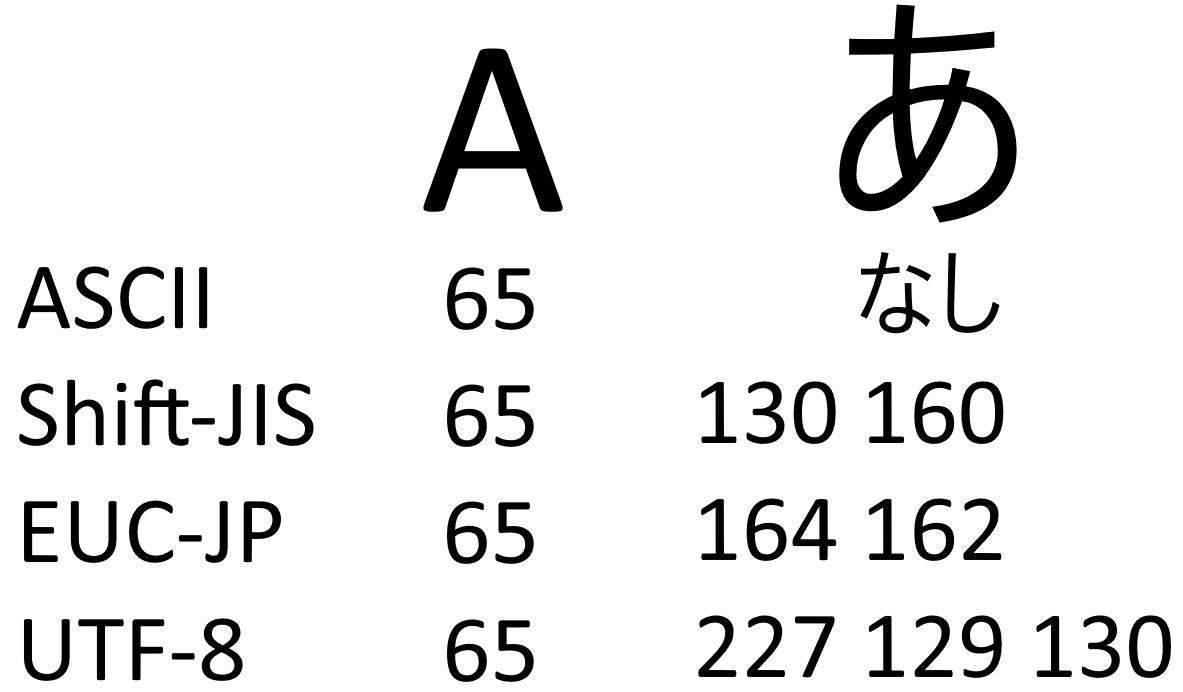
\includegraphics[width=0.65\textwidth]{slide08-img004.png}
    \end{figure}
\end{frame}

\begin{frame}[fragile]
	\frametitle{文字コードについて知ろう:テキスト P.\pageref{1:P:charCode}-P.\pageref{1:P:scraping}~~~\raisebox{-3mm}{
\includegraphics[width=0.1\textwidth]{raspberry}}}
    \large\textbf{P.\pageref{1:P:charCode}のASCIIコード表を見てみましょう}\\
    \begin{minipage}{0.55\textwidth}
        \begin{itemize}
            \item Decimalは10進数の数字、Hex(Hexadecimal)は16進数の数字、Char(Character)は文字を表します。
            \item 10進数は10数えたら位があがるように、16進数は16数えたら位が上がります。\\16進数では、0,1,2,3,4,5,6,7,8,9,A,B,C,D,E,Fを使って数を表します。
        \end{itemize}
    \end{minipage}
    \hfill
    \begin{minipage}{0.4\textwidth}
        {\upshape
            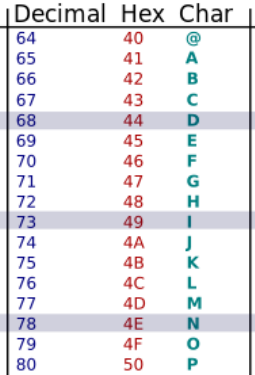
\includegraphics[height=0.7\textheight]{slide08-img005.png}}
    \end{minipage}
\end{frame}

\begin{frame}[fragile]
	\frametitle{文字コードについて知ろう:テキスト P.\pageref{1:P:charCode}-P.\pageref{1:P:scraping}~~~\raisebox{-3mm}{
\includegraphics[width=0.1\textwidth]{raspberry}}}
      \large\textbf{教科書をよみながら、例題をやってみよう}
				\begin{itemize}
					\item \ref*{1:E:ASCII}
					\item \ref*{1:E:UTF8}
					\item \ref*{1:E:iconv}
				\end{itemize}
      \vfill
      \large\textbf{速く終わった子は、次の問題をやってみよう}
				\begin{itemize}
					\item \ref*{1:Q:myName}, \ref*{1:Q:friendName}, \ref*{1:Q:emoticon}
					\item \ref*{1:Q:myNameUTF8}, \ref*{1:Q:friendNameUTF8}
				\end{itemize}
      \vfill
      \large\textbf{わからないことは、放っておかず、すぐに TA に聞きましょう}
\end{frame}

